\documentclass[11pt,a4paper]{ivoa}
\input tthdefs

\usepackage{xspace}
% Standard terms used throughout the document,
% defined as macro commands to maintain consistency

% Using non-breaking space character.
% https://stackoverflow.com/a/1012891

\newcommand{\xml} {XML}
\newcommand{\json} {JSON}
\newcommand{\yaml} {YAML}

\newcommand{\datamodel} {data~model}
\newcommand{\webservice} {webservice}
\newcommand{\webbrowser} {web browser}

\newcommand{\ivoa} {IVOA}
\newcommand{\uws} {UWS}
\newcommand{\vospace} {VOSpace}

\newcommand{\execplanner} {ExecutionPlanner}
\newcommand{\execworker} {ExecutionWorker}
\newcommand{\executionplanner} {Execution~Planner}

\newcommand{\jupyter} {Jupyter}
\newcommand{\jupyterhub} {JupyterHub}
\newcommand{\binderhub} {BinderHub}
\newcommand{\jupyternotebook} {Jupyter notebook}

\newcommand{\esap} {ESAP}
\newcommand{\escape} {ESCAPE}
\newcommand{\datalake} {DataLake}
\newcommand{\rucio} {Rucio}

\newcommand{\python} {Python}

\newcommand{\apache} {Apache}
\newcommand{\spark} {Spark}
\newcommand{\pyspark} {PySpark}
\newcommand{\zeppelin} {Zeppelin}

\newcommand{\ocicontainer} {OCI~container}
\newcommand{\docker} {Docker}
\newcommand{\dockercompose} {Docker compose}
\newcommand{\dockercontainer} {Docker container}

\newcommand{\openstack} {Openstack}
\newcommand{\kubernetes} {Kubernetes}

\newcommand{\codeword}[1] {\texttt{#1}}
\newcommand{\footurl}[1] {\footnote{\url{#1}}}

\newcommand{\dataset} {dataset}
\newcommand{\datascience} {data~science}
\newcommand{\scienceplatform} {science~platform}

\newcommand{\executable} {\textit{executable}}
\newcommand{\executablething} {\textit{executable}~thing}
\newcommand{\excutabletask} {\textit{executable} task}
\newcommand{\workerjob} {\textit{job}}

\newcommand{\cpu} {CPU}
\newcommand{\gpu} {GPU}
\newcommand{\nvidiagpu} {NVIDIA~AD104~GPU}

\newcommand{\job} {\textit{job}}
\newcommand{\task} {task}

\newcommand{\scalable} {scalable}

\usepackage{listings}
\usepackage{xcolor}

%\colorlet{punct}{red!60!black}
\colorlet{numb}{magenta!60!black}
\definecolor{html-gray}{HTML}{EEEEEE}
\definecolor{light-gray}{gray}{0.95}
\definecolor{delim}{RGB}{20,105,176}

\lstset{
    basicstyle=\small\ttfamily,
    columns=fullflexible,
    frame=none,
    backgroundcolor=\color{light-gray},
    stepnumber=1,
    %numbers=left,
    numbers=none,
    numberstyle=\small,
    numbersep=8pt,
    %xleftmargin=\parindent,
    xrightmargin=1cm,
    showstringspaces=false,
    keepspaces=true,
    breaklines=true,
    linewidth=14cm,
    frame=none
}

% https://tex.stackexchange.com/questions/83085/how-to-improve-listings-display-of-json-files
% https://tex.stackexchange.com/a/83100
% https://tex.stackexchange.com/questions/10828/indent-a-code-listing-in-latex
% https://tex.stackexchange.com/a/10831
\lstdefinelanguage{json}{
    literate=
     *{0}{{{\color{numb}0}}}{1}
      {1}{{{\color{numb}1}}}{1}
      {2}{{{\color{numb}2}}}{1}
      {3}{{{\color{numb}3}}}{1}
      {4}{{{\color{numb}4}}}{1}
      {5}{{{\color{numb}5}}}{1}
      {6}{{{\color{numb}6}}}{1}
      {7}{{{\color{numb}7}}}{1}
      {8}{{{\color{numb}8}}}{1}
      }

\lstdefinelanguage{yaml}{
    literate=
     *{0}{{{\color{numb}0}}}{1}
      {1}{{{\color{numb}1}}}{1}
      {2}{{{\color{numb}2}}}{1}
      {3}{{{\color{numb}3}}}{1}
      {4}{{{\color{numb}4}}}{1}
      {5}{{{\color{numb}5}}}{1}
      {6}{{{\color{numb}6}}}{1}
      {7}{{{\color{numb}7}}}{1}
      {8}{{{\color{numb}8}}}{1}
      }

\hyphenation{Exe-cut-able-Thing}

\title{IVOA Execution Planner}

% see ivoatexDoc for what group names to use here; use \ivoagroup[IG] for
% interest groups.
\ivoagroup{GWS}

\author[http://www.ivoa.net/twiki/bin/view/IVOA/DaveMorris]
       {Dave Morris}

\editor[http://www.ivoa.net/twiki/bin/view/IVOA/DaveMorris]
       {Dave Morris}

% \previousversion[????URL????]{????Concise Document Label????}
\previousversion{This is the first public release}

\begin{document}
\begin{abstract}
\label{abstract}

One of the long term goals of the IVOA has been to enable users to
move the code to the data.
This is becoming more and more important as the size and complexity
of the \dataset{}s available in the VO increases.
%\citep{gaia-at-esac}
%\footurl{https://www.skao.int/en/explore/big-data}
%\footurl{https://www.lsst.org/scientists/keynumbers}

The \ivoa{} \executionplanner{} provides a step towards making this possible.

The \ivoa{} \executionplanner{} is designed to address a specific question;
given an executable thing, e.g. a \python{} program or a \jupyternotebook{},
what facilities are available to run it?

To do this, the \ivoa{} \executionplanner{} specification defines
a data model for describing the executable thing
and the resources needed to execute it,
and a \webservice{} API for finding platforms
that are able to execute it.

Together these components enable a user to ask a simple question
\textit{"Where (and when) can I execute my program?"}

This in turn enables users to move code between \scienceplatform{}s.
Allowing them to develop their code on one platform and then apply it to a different
\dataset{} by sending it to execute on another platform.

\end{abstract}

\section*{Acknowledgments}
\label{acknowledgments}

The authors would like to thank all the participants in the IVOA and ESCAPE projects
who have contributed their ideas, critical reviews, and suggestions to this document.

\section*{Conformance-related definitions}

The words ``MUST'', ``SHALL'', ``SHOULD'', ``MAY'', ``RECOMMENDED'', and
``OPTIONAL'' (in upper or lower case) used in this document are to be
interpreted as described in IETF standard RFC2119\citep{std:RFC2119}.

The \emph{Virtual Observatory (VO)} is a general term for a collection of
federated resources that can be used to conduct astronomical research,
education, and outreach.
The \href{https://www.ivoa.net}{International Virtual Observatory Alliance (IVOA)}
is a global collaboration of separately funded projects to develop standards and
infrastructure that enable VO applications.

\section{Introduction}
\label{introduction}

The \ivoa{} \executionplanner{} specification defines two \webservice{} interfaces,
the \execplanner{} and the \execworker{}, and a common \datamodel{} for describing
executable tasks.

Together these provide a common interface for service discovery, resource allocation
and execution scheduling across a heterogeneous federation of different types of
execution platform.

\begin{itemize}
    \item \execplanner{} \webservice{} – a discovery service to find execution platforms, allocate resources and schedule execution.
    \item \execworker{} \webservice{} – an asynchronous service for executing tasks (based on the \ivoa{} \uws{} pattern).
    \item \execplanner{} \datamodel{} – a common data model for describing an executable thing and its resource requirements.
\end{itemize}

\subsection{Role within the VO Architecture}
\label{subsec:ivoarole}

% As of ivoatex 1.2, the architecture diagram is generated by ivoatex in
% SVG; copy ivoatex/archdiag-full.xml to role_diagram.xml and throw out
% all lines not relevant to your standard.
% Notes don't generally need this.  If you don't copy role_diagram.xml,
% you must remove role_diagram.pdf from SOURCES in the Makefile.
\begin{figure}
\centering
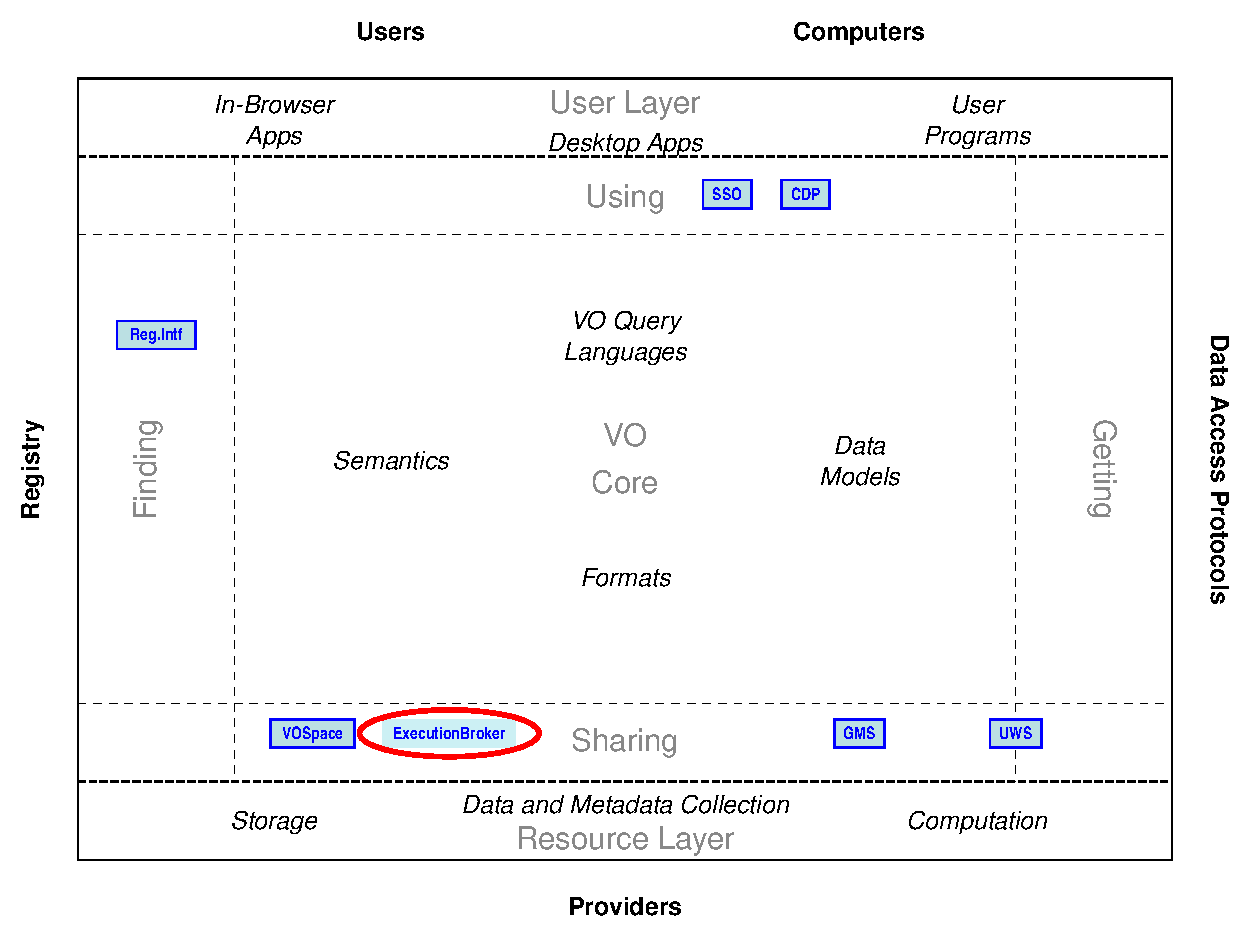
\includegraphics[width=0.9\textwidth]{role_diagram.pdf}
\caption{Architecture diagram showing the \ivoa{} \executionplanner{}'s role in the \ivoa}
\label{fig:archdiag}
\end{figure}

The IVOA Architecture\citep{2010ivoa.rept.1123A} provides a high-level view of how IVOA
standards work together to connect users and applications with providers of data
and services.
Fig.~\ref{fig:archdiag} shows the role the \ivoa{} \executionplanner{} plays within the this architecture.

In response to the increasing size and complexity of the next generation of science \dataset{}s
a number of \ivoa{} members are developing intergrated \scienceplatform{}s which bring
together the \dataset{}s co-located with the compute resources needed to analyse them.
\footurl{https://data.lsst.cloud/}
\footurl{https://rsp.lsst.io/index.html}

The \scienceplatform{}s make extensive use of the \ivoa{} data models and
vocabularies to describe their \dataset{}s, and use the \ivoa{} data access
services to find and access data from other data providers.
In addition, some of the \scienceplatform{}s use \ivoa{} \vospace{} services to manage
data transfers to and from local storage co-located with the compute resources.

However, to date the \ivoa{} does not provide any APIs or \webservice{} interfaces that
enable \scienceplatform{}s to exchange the software used to analyse the data.
The \ivoa{} \executionplanner{} provides a step towards making this possible.

This places the \ivoa{} \executionplanner{} in the same region of the \ivoa architecture
as the \ivoa{} \vospace{} specification\citep{2009ivoa.specQ1007G},
providing an infrastructure level service that enables service discovery,
resource allocation and execution scheduling across a heterogeneous federation
of execution platforms.

The \ivoa{} \executionplanner{} specification refers to the
\ivoa Single-Sign-On standard\citep{2017ivoa.spec.0524T}
for authentication (see section xx )%\ref{subsec:authentication}
and the
\ivoa Credential Delegation Protocol\citep{2010ivoa.spec.0218P}
for delegating credentials to other services.

The \ivoa{} \executionplanner{} specification also describes how to register
an \execplanner{} service in the
\ivoa{} Registry\citep{2009ivoa.spec.1104B}
making it findable within the wider context of the VO.

\subsection{Executable things}
\label{executablething}

To understand the problem that \ivoa{} \executionplanner{} is trying to solve
it is useful to describe what an \executablething{} is in this context.
In general terms, this document refers to something that can be executed, or run,
as an \executable.

To explain what this means we can start with a science domain function that we want to perform.
For example, the mathematical concept of the square root of a number.
We can calculate the square root of a positive number using the Newton–Raphson
algorithm\footurl{https://en.wikipedia.org/wiki/Newton\%27s_method}
which produces successively closer approximations to the result.
However, in general case, this mathematical description of the algorithm would not be considers as an \executablething.

We can write a \python{} program to use this algorithm to calculate the square root of a number.
This is the first identifiable \executablething{} in our example.
To be able to use this \executablething{}, you would need a computing resource with the appropriate
hardware and software environment. In this case, a computing resource with the \python{} interpreter
installed along with any 3rd \python{} modules required by the program.
This environment is often referred to as the \python{} runtime.

In the context of \scienceplatform{}s and \datascience{}, a common pattern is to provide this environment
using an \ocicontainer{}\footurl{https://opencontainers.org/},
or \dockercontainer\footurl{https://docs.docker.com/get-started/what-is-a-container/},
to package the \python{} program and the \python{} runtime together as a single binary object.
This package, or container, is itself an \executablething{}. One which requires a different execution
environment than the original \python{} program.
The aim of containerization is to package \executablething{}s together with the software environment
they need as single binary object that interfaces with a standard execution environment,
referred to as the \textit{container runtime} or \textit{container engine}.
To be able to use this \executablething{}, you would need a computing resource with the appropriate
hardware and software environment. In this case, a computing resource with the OCI container runtime installed.

We could also create a \jupyternotebook{} that demonstrates how to use our \python{} program.
This is the third \executablething{} in our example.
One which provides an interactive environment for the user to experiment with.
As before, to be able to use this \executablething{}, we would need a computing resource with
the appropriate hardware and software environment.
In this case, a computer with the \jupyternotebook{} platform installed along with all the 3rd \python{} modules
needed by our \python{} program.
In the context of \scienceplatform{}s and \datascience{}, a common pattern is to provide this environment as a \webservice{}
that allows the user to connect to the \jupyternotebook{} via a \webbrowser.

From one algorithm that implements a science domain function, we have created three different \executablething{}s.
A \python{} program, an \ocicontainer{} packaging the \python{} program and its dependencies, and an interactive \jupyternotebook{}
that demonstrates how to use the \python{} progran.
Each of which requires a different computing environment to execute.
A basic \python{} runtime, the \ocicontainer{} runtime, and a \jupyternotebook{} service.

We may also want to consider the data that we are applying the algorithm to.
If we are learning how to use algorithm, then a basic computing resource will be sufficient
to experiment with.
However, if we have a \dataset{} of ten million numbers that we want to process, then we may
need to consider adding extra storage to handle the input data and the results.
For a large \dataset{} it may also be worth using a \gpu{} to accelerate the calculation steps
for such a large \dataset{}.

The \ivoa{} \executionplanner{} \datamodel{} provides a way to describe what each of these \executablething{}s
are and what resources are needed to execute them.
This can include things like number of \cpu{} cores and amount of memory it needs,
whether it needs a \gpu{}, the location of the input data, the storage space needed to perform
the calculation and the storage space needed to save the results.
This description can be passed to an \ivoa{} \executionplanner{} service to
discover if the service is able to provide the resources required to execute it.

\section{Client-server conversation}
\label{conversation}

The core idea behind the \ivoa{} \executionplanner{} is based on a conversation between the client
and the \execplanner{} services to discover where, how, and when, an \executablething{} can be
executed.

The conversation starts with the client sending a description of the \executablething{} to the
\execplanner{} services, each of which respond with a top level \codeword{YES|NO} answer, and if
the answer is \codeword{YES}, a list of offers describing how the \excutabletask{}
can be executed on their platform.

\begin{lstlisting}[]
Request  - Can this platform execute <task> ?
Response - YES, list of <offer>[]
\end{lstlisting}

The client can then choose which of the offers it wants to use and sends a reply
to that \execplanner{} service accepting the offer.
In response the \execplanner{} will mark the resources in the offer as reserved,
initiate a \workerjob{} in an \execworker{} service to execute the task
and reply with details of how to access it.

\begin{lstlisting}[]
Request  - I accept <offer>[n]
Response - <job details>
\end{lstlisting}

The client can then uses the connection details in the \workerjob{} response to contact
the \execworker{} service and track its status.
For further details of the \webservice{} request and response messages see section xxx.

Note that the client does not need to cancel the offers made by the other \execplanner{} services.
Offers are only valid for a limited period of time, and expire naturally when they reach the end
of their lifetime.

The content of the messages can be explained as a series of questions that
a client would ask to discover if the platform has the resources available
to execute the task.

Each of these questions becomes part of the request sent to the \execplanner{}
\webservice{} and part of the response.

\subsection{Level 1 - the \executable{}}
\label{executable}

At the simplest level the client just needs to check whether a platform is able to execute a particular
type of \excutabletask{}.
For example, \textit{"Is this platform able to run a \jupyternotebook{}?"}

In order to do this, the request needs to specify the task type, e.g. \jupyternotebook{},
along with details about it, e.g. where to fetch the notebook from.

The informations in this part of the description us different for each type of \executable{}.
Rather than try to model every possible type of \executable{} in one large \datamodel{},
the \datamodel{} for each type is described by an extension to the core \datamodel{}.

To support this pattern the core \executionplanner{} \datamodel{} has two fields, \codeword{type},
a URI identifying the type of \executable{}, and \codeword{spec}, a place holder for
type specific details.

\begin{lstlisting}[]
executable:
  # A URI identifying the type of executable.
  # e.g.
  # https://www.purl.org/ivoa.net/ep/task-type/oci-container
  # https://www.purl.org/ivoa.net/ep/task-type/jupyter-notebook
  type: "https://www.purl.org/ivoa.net/ep/task-type/example"

  # The details, specific to the type of executable.
  spec: {}
\end{lstlisting}

The \datamodel{} extension for each type of \executable{} defines the metadata needed to
describe that particular type.
For example, the \datamodel{} extension for a \jupyternotebook{} needs to describe where
to fetch the source code for the notebook from.
\begin{lstlisting}[]
executable:
  # A URI identifying the type of executable.
  type: "https://www.purl.org/ivoa.net/ep/task-type/jupyter-notebook"

  # The details, specific to a jupyter-notebook task.
  spec:
    notebook: "https://.../example.jpnb"
\end{lstlisting}

It may also include a reference to a \codeword{requirements.txt} file that describes any additional \python{}
libraries needed to run the notebook.
\begin{lstlisting}[]
executable:
  # A URI identifying the type of executable.
  type: "https://www.purl.org/ivoa.net/ep/task-type/jupyter-notebook"

  # The details, specific to a jupyter-notebook task.
  spec:
    notebook: "https://.../example.jpnb"
    requirements: "https://.../requirements.txt"
\end{lstlisting}

The \datamodel{} extension for an \ocicontainer{} needs to describe what operating system and system architecture
the container is is built for, and where to fetch the binary image from.

\begin{lstlisting}[]
executable:
  # A URI identifying the type of executable.
  type: "https://www.purl.org/ivoa.net/ep/task-type/oci-container"

  # The details, specific to an oci-container task.
  spec:
    os:    "linux"
    arch:  "amd64"
    repo:  "ghcr.io"
    image: "ivoa/oligia-webtop"
    version: "ubuntu-2022.01.13"
\end{lstlisting}

The \executionplanner{} specification defines an initial set of common task types, e.g. \ocicontainer{}, \jupyternotebook{},
and \zeppelin{} notebook.
The extension pattern is designed to make it easy for 3rd parties to develop new types of tasks appropriate for their science domain.

Using the \codeword{type} URI to identify the task type means that service implementations do not need to understand
all of the different possible types of \executable{} that a client could request.
If a service that doesn’t recognize a particular type, it can simply reply \codeword{NO}.

\begin{lstlisting}[]
Request  - Can this platform execute <unkown-type> ?
Response - NO
\end{lstlisting}

For a full listing of the task types included see appendix xxx.

TODO some text about using URIs ...

\subsection{Level 2 - the resources}
\label{resources}

At the next level the client may need to check whether a platform has sufficient compute resources
needed to execute a particular \excutabletask{}.
For example, \textit{"Can this platform provide enough resources to run this \jupyternotebook{}?"}

\subsubsection{Level 2a - compute resources}
\label{compute-resources}

In order to do this the request would not only need to describe the \executable{} itself,
but also the minimum level of compute resources needed in terms of \cpu{} cores, memory, \gpu{}s
and disc space needed to execute it.

The \datamodel{} for describing compute resources is, in most cases, common to all types of \executable{},
so the \datamodel{} for these requirements are defined as part of the core \executionplanner{} \datamodel{}.

It is important to note that all of the resource requirements are optional.
As in the example from the previous section, a request to execute a simple \jupyternotebook{}
would not need to include any resource details.

\begin{lstlisting}[]
executable:
  # A URI identifying the type of executable.
  type: "https://www.purl.org/ivoa.net/ep/task-type/jupyter-notebook"

  # The details, specific to a jupyter-notebook task.
  spec:
    notebook: "https://.../example.jpnb"
\end{lstlisting}

As long as this \jupyternotebook{} only needs a minimal set of resources to run, e.g.
2 \cpu{} cores, 2G of memory and 20G of disc space, then this task probably doesn't need
any additional resources.

However, if this \jupyternotebook{} needs a specific type of \gpu{} to function properly,
then can be added to the request by specifying a compute resource with the specific type
of \gpu{}.

\begin{lstlisting}[]
# Details of the executable.
executable:
  # A URI identifying the type of executable.
  type: "https://www.purl.org/ivoa.net/ep/task-type/jupyter-notebook"
  # The details, specific to a jupyter-notebook task.
  spec:
    notebook: "https://.../example.jpnb"

# Details of the resources needed.
resources:
  compute:
  - name: "example-one"
    type: "https://.../generic-compute"
    spec:
      gpu:
        # A URI identifying the type of GPU.
        type: "https://www.techpowerup.com/gpu-specs/nvidia-ad104.g1013"
\end{lstlisting}
%TODO purl URI for the GPU type.

With this detail added to the request, platforms that are not able to provide this kind of \gpu{}
would simply reply \codeword{NO}.

\begin{lstlisting}[]
Request  - Can this platform provide a compute resource with a 'NVIDIA~AD104~GPU' ?
Response - NO
\end{lstlisting}

Note that a platform does not need to know what a  "\nvidiagpu{}" is to be able to reply with a sensible aswer.
If a platform receives a request for resource requirement that it don't understand, it should simply reply \codeword{NO}.

\begin{lstlisting}[]
Request  - Can this platform provide an <unknown thing> ?
Response - NO
\end{lstlisting}

The only platforms that will reply \codeword{YES} are ones that understand what a "\nvidiagpu{}"
is and are able to provide compute resources with one.

The \datamodel{} for the \gpu{} resource follows the same pattern as the \datamodel{} for
the \executable{}. The \datamodel{} defines a \codeword{type} URI to identify the type of \gpu{},
and a \codeword{spec} section for type specific details,
e.g. the minimum amount of memory and number of shaders.

\begin{lstlisting}[]
# Details of the executable.
executable:
  ....
# Details of the resources needed.
resources:
  compute:
  - name: "example-one"
    type: "https://.../generic-compute"
    spec:
      gpu:
        # A URI identifying the type of GPU.
        type: "https://www.techpowerup.com/gpu-specs/nvidia-ad104.g1013"
        # The details, specific to a 'NVIDIA~AD104~GPU'.
        spec:
          minmemory: 20
          minshaders: 6144
\end{lstlisting}

\subsubsection{Level 2b - minimum and maximum}
\label{minandmax}

The \datamodel{} for describing compute resources includes elements for specifying the numeric size
and number of resources such as \cpu{} cores, memory and storage.

If the \jupyternotebook{} in our example needs a minimum of 8 \cpu{} cores and 16G bytes of memory
to be able to perform its calculations, then this can be specified in the required compute resources.

\begin{lstlisting}[]
# Details of the executable.
executable:
  ....
# Details of the resources needed.
resources:
  compute:
  - name: "example-one"
    type: "https://.../generic-compute"
    spec:
      mincores:   8
      minmemory: 16
\end{lstlisting}

All of the \datamodel{} elements for specifying the size or number of compute resources are defined
as pairs of minimum and maximum values.
This allows a conversation to occur between the \execplanner{} client and services
to discover the best platform to execute the task.

The client requests the minimun resources it needs,
and each service responds with a set of offers which specify the maximum
level of resources it can offer.

For example, if a platform is able to provide double the compute resources,
16 \cpu{} cores and 32G bytes of memory,
then it can indicate this by specifying higher maximum values in its response.

\begin{lstlisting}[]
# Details of the executable.
executable:
  ....
# Details of the resources needed.
resources:
  compute:
  - name: "example-one"
    type: "https://.../generic-compute"
    spec:
      mincores:   8
      maxcores:  16
      minmemory: 16
      maxmemory: 32
\end{lstlisting}

This response represents an offer to start with a minimum of 8 \cpu{} cores and 16G of memory
as requested, with the option to use a maximum of 16 \cpu{} cores and 32G of memory if needed.

This \scalable{} compute resource represents something like a \kubernetes{} platform where the
execution can start with a minimum configuration and scale on demand up to a maximum limit.

This is slightly different to a platform like \openstack{} which allocates resources
in specific blocks, defined by the set by the set of virtual machine \textit{'flavors'}
available on that paerticular platform.
If the smallest flavor of virtual machine available on the platform has 16 \cpu{} cores and 24G of memory,
then the service can represent that by making an offer with higher minimum values.

\begin{lstlisting}[]
# Details of the executable.
executable:
  ....
# Details of the resources needed.
resources:
  compute:
  - name: "example-one"
    type: "https://.../generic-compute"
    spec:
      mincores:  16
      maxcores:  16
      minmemory: 24
      maxmemory: 24
\end{lstlisting}

This response represents an offer to start with a fixed allocation of 16 \cpu{} cores and 24G of memory.

An \execplanner{} MAY NOT make an offer with less than the minimum resources requested.
For example, if an \openstack{} platform only has a tiny virtual machine flavor available,
with only 1 \cpu{} core and 2G of memory, then it MAY NOT offer this resource it it is less than
the requested minimum.

Note that the term \textit{'compute resource'} specifically avoids stating whether the the
notebook is run in a \openstack{} virtual machine or a \kubernetes{} cluster.
As far as the user is concerned, it doesn't matter, as long as the compute resource provides
sufficient \cpu{} cores and memory for their notebook to execute.

%IF the task requires a specific type of compute resource it can be specified
%in the type URI.

Full details of the \datamodel for decribing compute resources is given in section xx.

\subsubsection{Level 2c - storage resources}
\label{storage-resources}

The resources section of the request can also be used to specify storage resources.

There are two main types of storage resources:
\begin{itemize}
    \item External storage resources that are managed by an external provider.
    \item Internal storage resources that are managed by the platform.
\end{itemize}

Within that there are two types of internal storage resources:
\begin{itemize}
    \item Ephemeral storage managed by the platform, available for the duration of the \job{}, created when the \job{} start and released as soon as the \job{} is completed.
    \item Persistent storage managed by the platform that exists beyond the lifetime of the \job{}, created before the \job{} starts and remaining after the \job{} has been completed.
\end{itemize}

The simplest of these are ephemeral storage resources managed by the execution platform.
For example, if the \jupyternotebook{} in our example requires 1Tbyte of space to perform its calculations,
then this can be specified in the request by defining an ephemeral storage resource.

\begin{lstlisting}[]
# Details of the executable.
executable:
  ....
# Details of the resources needed.
resources:
  ....
  storage:
  - name: "scratch-space"
    type: "https://.../ephemeral"
    spec:
      size: 1024
\end{lstlisting}

To enable the \jupyternotebook{} to access this storage, we need to add a
corresponding \codeword{volume} element to the compute resource that describes
where to mount the storage resource.

For example, the following specification defines a 1Tbyte ephemeral storage resource
and mounts it at \codeword{/temp} in the filesystem of the compute resource.

\begin{lstlisting}[]
# Details of the executable.
executable:
  ....
# Details of the resources needed.
resources:
  ....
  compute:
  - name: "example-one"
    ....
    volumes:
    - name: "scratch-space"
      path: "/temp"
      mode: "rw"
  storage:
  - name: "scratch-space"
    type: "https://.../ephemeral"
    spec:
      size: 1024
\end{lstlisting}

This part of the \executionplanner{} \datamodel{}, separating the details of how
a storage resource is implemenmted from the details of how is mounted inside a
computing resource, is based on a pattern used by \kubernetes{} to describe storage
volumes and their mount points within containers.

This pattern can also be used to define a storage resource that imports data from
an external source.
For example, if the user wanted to use the \jupyternotebook{} to analyse data stored
in an external S3 system, this can be done by defining an external storage resource
that describes where the data is,
and a corresponding volume mount inside the compute resource.

\begin{lstlisting}[]
# Details of the executable.
executable:
  ....
# Details of the resources needed.
resources:
  ....
  compute:
  - name: "example-one"
    ....
    volumes:
    - name: "source-data"
      path: "/data"
      mode: "r"
  storage:
  - name: "source-data"
    type: "https://.../amazon-S3"
    spec:
      endpoint: "https://.../echo"
      bucket: "example-data"
\end{lstlisting}

Again, this pattern of separating how the data is stored outside the system
and how it appears inside the compute resource borrows heavily from the
pattern used by \kubernetes{} to describe Persistent Volumes (PV) and
Persistet Volume Claims (PVC).

The same pattern can be used to describe a storage resource that can be used
to save the analysis results, by defining a persistent storage resource
allocated by the system, and a corresponding volume mount inside the compute resource.

\begin{lstlisting}[]
# Details of the executable.
executable:
  ....
# Details of the resources needed.
resources:
  ....
  compute:
  - name: "example-one"
    ....
    volumes:
    - name: "results"
      path: "/results"
      mode: "rw"
  storage:
  - name: "results"
    type: "https://.../persistent"
    spec:
      minlifetime: "1D"
      minsize: 100
\end{lstlisting}

By setting the storage resource type to \codeword{https://.../persistent},
the client is asking the \execplanner{} service to take care of allocating
the storage and managing its lifecycle.
It is up to the \execplanner{} service to decide how to store the data and
make it accessible to the user.

For example, an execution platform may have a \rucio{} storage system which
it uses to store user generated data.
In which case the \execplanner{} service would respond with an offer that
stores the results in the \rucio{} system and provides details of how the user
can access it after the \job{} has completed.

\begin{lstlisting}[]
# Details of the executable.
executable:
  ....
# Details of the resources needed.
resources:
  ....
  compute:
  - name: "example-one"
    ....
    volumes:
    - name: "results"
      path: "/results"
      mode: "rw"
  storage:
  - name: "results"
    type: "https://.../rucio"
    spec:
      minlifetime: "1D"
      maxlifetime: "5D"
      minsize:  100
      maxsize:  200
      endpoint: "http://...."
      objectid: "cdc78e7d-8032-497e-9a5b-01c720ea2223"
      lifecycle: "managed"
\end{lstlisting}

In this example, the client requested at least 100G bytes of storage available for 1 day
and in response the service is offering up to 220G bytes available for 5 days stored in a
\rucio{} system.
It is up to the client to decide if it can access the particular \rucio{} system described
in the response.

Making an offer with the lifecycle set to \codeword{managed} and a lifetime of \codeword{5D}
means that the service will manage the lifecycle automatically.
The storage will be avalable for 5 days after the \job{} completes and then it will be deleted.
The client doesn't need to worry about tidying up afterwards.

It is important to note that at this point in time the storage is proposed, but not yet allocated.
The persistent storage is only allocated if the client accepts this particular offer.
This allows an \execplanner{} service to make multiple offers with different options for the
persistent storage, allowing the client to select and accept the one that best fits its use case.

The same \datamodel can be used the other way around as well.
If the client already knows where it wants the data to be stored, for example at a specific
\vospace{} location, then it can spcify this in the request.

\begin{lstlisting}[]
# Details of the executable.
executable:
  ....
# Details of the resources needed.
resources:
  ....
  compute:
  - name: "example-one"
    ....
    volumes:
    - name: "results"
      path: "/results"
      mode: "rw"
  storage:
  - name: "results"
    type: "https://.../vospace"
    spec:
      endpoint: "http://...."
      path: "/experiment-21/results"
      lifecycle: "unmanaged"
\end{lstlisting}

It is up to the \execplanner{} service to work out if is able to access the
\vospace{} location and mount it as a volume in the compute resource,
using either its own authentication, or a delegated form of the authentication
provided by the client.

If it can access the \vospace{} location, then the \execplanner{} server responds
with an offer, otherwise if it can't access the \vospace{} location for whatever
reason the \execplanner{} would respond with \codeword{NO}.

Note that in this example, the client has specified the lifecycle as \codeword{unmanaged},
which means that the \execplanner{} is not involved in managing the creation or deletion
of the data in \vospace.
It is aloso possible for the client to ask the \execplanner{} service to manage
data in an external resource.

\begin{lstlisting}[]
....
resources:
  ....
  storage:
  - name: "results"
    type: "https://.../vospace"
    spec:
      endpoint: "http://...."
      path: "/experiment-21/results"
      lifecycle: "managed"
      maxlifetime: "2D"
\end{lstlisting}

In this example, the client is specifying an external \vospace{} location to store the data,
but it is asking the \execplanner{} service to manage the lifecycle, creating the location
in \vospace{} at the start of the \job{} and deleting it 2 days after the \job{} completes.

This kind of negotiation over who is responsible for creating and deleteing storage resources
enables a client to put together a workflow of interconnected steps. With the services
managing the lifecycle of the resources, releasing them automatically after the
specified length of time.

\subsection{Level 3 - authentication}
\label{authentication}

At the next level the client may need to check whether the user account making the request
has sufficient access rights and resource quota needed to execute a particular \excutabletask{}.
Equivalent to asking:
\textit{"Do I have permission to use these resources to run this \jupyternotebook{}?"}

There are two ways for the \execplanner{} service to check the user's identity.
The implicit method is for the client to authenticate to the \webservice as normal
and the \execplanner{} service will use that identity to check for access rights
to execute the \job{}.

The \datamodel{} also allows for an explicit statement of identity in the request.
The \datamodel{} for authentication follows the same pattern as the other sections,
defining a \codeword{type} URI to identify the type of authentication method,
and a \codeword{spec} section for the type specific details.

For example, to explicitly include basic authentication with username and password
in the request:
\begin{lstlisting}[]
....
authentication:
- name: "basic-auth"
  type: "https://.../basic"
  spec:
    username: "..."
    password: "..."
\end{lstlisting}

This \datamodel allows the client to supply multiple authentication methods
in the request. The \execplanner selects the authentication methods it
accepts from those in the request and includes the name and type of the
methods that it accepts in its reply.

For example, if the client supplies both basic and token authentication
in the request:
\begin{lstlisting}[]
....
authentication:
- name: "basic-auth"
  type: "https://.../basic"
  spec:
    username: "..."
    password: "..."
- name: "token-auth"
  type: "https://.../token"
  spec:
    token: "..."
\end{lstlisting}

If the \execplanner service accepted both these methods, it would include the
name and type of the accepted methods in its reply, along with enough non-secret
information from the \codeword{spec} to identify the authenticated identity.
\begin{lstlisting}[]
....
authentication:
- name: "basic-auth"
  type: "https://.../basic"
  spec:
    username: "..."
- name: "token-auth"
  type: "https://.../rfc7519"
  spec:
    sub: "..."
\end{lstlisting}

If the original \webservice call to the \execplanner service is authenticated,
then the \execplanner should include a reference to the implicit authentication
in its reply.

\begin{lstlisting}[]
....
authentication:
- name: "http-request"
  type: "https://.../oidc"
  spec:
    identity: "..."
\end{lstlisting}

The result is that an offer made by an \execplanner service includes details of the
authenticated identities that are allowed to use the offer on that service.

If the original question is equivalent to:
\textit{"Do \textbf{these identities} have sufficient access rights and quota to run this \jupyternotebook{}?"}

Then the response from the \execplanner service is equivalent to:
\textit{"This offer asserts that \textbf{these identities} have sufficient access rights and quota to run this \jupyternotebook{}?"}

The client should use one of the authentication methods listed in the offer when
they contact the \execplanner service to accept the offer and start the \job{}.
They should then continue to use the same authentication method when making subsequent
requests to the \execworker{} service to access the \job{} status and results.

The \executionplanner specification defines an initial set of authentication methods
corresponding to the methods defined in the
\ivoa Single-Sign-On standard\citep{2017ivoa.spec.0524T}

\begin{itemize}
    \item ....
    \item ....
\end{itemize}

However, the \datamodel also allows an \execplanner service to accept authentication
methods that are not covered by the \ivoa SSO specification.
A client is free to use any authentication method, including one not covered by the
\ivoa SSO specification. It is up to the \execplanner service to decide how it
handles the authentication infomation supplied.

This means that the \executionplanner can be deployed in other domains outside the \ivoa,
without explicitly requiring the project to adopt the \ivoa SSO specification.

\subsection{Level 4 - Date and time}
\label{date-time}

The \codeword{datetime} part of the \datamodel enables the client and server to have a
conversation about when a \job{} can be executed.

The client can specify one or more time periods when it would like to start the \job{},
and the minimum duration that it thinks would be needed to complete the \job{}.

The \execplanner{} service may respond with one more offers that specify when the \job{}
would start and the maximum duration that the \job{} would be allowed to consume.
It is then up to the client to select which of the offers best suites the use case.

The start-time for a \job{} is expressed as an array of time intervals, as defined by
ISO 8601\citep{std:iso8601}
\footurl{https://www.iso.org/iso-8601-date-and-time-format.html}
\footurl{https://en.wikipedia.org/wiki/ISO_8601}.
Specifically, type 1 or type 2 intervals, excluding type 3 and 4 intervals
(duration and end, and duration only) and excluding repeats.

\begin{itemize}
    \item <start>/<end>
    \item <start>/<duration>
\end{itemize}

Note that the duration part of the interval applies to the start-time, specifying the
range of allowed start-times.

If no duration is specified, this means an absolute start-time;
e.g. the \job{} should start at 11:30 on the 14th August.
\begin{lstlisting}[]
....
datetime:
- start: "2023-08-14T11:30Z"
\end{lstlisting}[]

If the start and are specified, this means the start-time may be somewhere between
the start and end values;
e.g. the \job{} should start between 11:30 and 12:00on the 14th August.
\begin{lstlisting}[]
....
datetime:
- start: "2023-09-14T11:30Z/T12:00Z"
\end{lstlisting}[]

If a duration is specified, this means the start-time may be somewhere between the
start and the start plus the duration;
e.g. the \job{} will start between 11:30 and 12:00 on the 14th August.
\begin{lstlisting}[]
....
datetime:
- start: "2023-09-14T11:30Z/PT30M"
\end{lstlisting}[]

The \execplanner container may respond with one or more offers that start somewhere
within one of the ranges specified in the request.
The start-times in the offers may be more precise than the start-time in the request,
but they must all occur within one of the ranges specified in the request.

The maximum and minimum execution duration are expressed as time periods, as defined by ISO 8601.

For example, for the unattended batch mode execution of an \ocicontainer, the user might not be concerned about
when the \job{} starts, but they may want to specify the minimum duration needed to complete the task.

In which case, the client may simply request a minimum duration of 1 hour.
\begin{lstlisting}[]
....
datetime:
- minduration: "1H"
\end{lstlisting}[]

The \execplanner service may respond with one or more offers that start at different times and
set different values for the maximum duration.

It may offer a maximum duration of 1 hour starting at 11am on Monday the 14th.
\begin{lstlisting}[]
....
datetime:
- start: "2023-09-14T11:30Z"
  minduration: "1H"
  maxduration: "1H"
\end{lstlisting}[]

It may also offer a maximum of 2 hours execution starting between 10pm and 11pm.
\begin{lstlisting}[]
....
datetime:
- start: "2023-09-14T22:00Z/PT1H"
  minduration: "P1H"
  maxduration: "P2H"
\end{lstlisting}[]

If all of the other parameters are the same, compute and storage resources, then the
\execplanner{} service may offer more than one time slot in the same offer.

\begin{lstlisting}[]
....
datetime:
- start: "2023-09-14T11:30Z"
  minduration: "1H"
  maxduration: "1H"
- start: "2023-09-14T22:00Z/PT1H"
  minduration: "P1H"
  maxduration: "P2H"
\end{lstlisting}[]

If the client decides to accept this offer, they may specify which of the start-times
they want when they make the acceptance request.

Alternatively, the \execplanner{} service may make separate offers each with a different start-time.

For example, if the client asks for 2 cores and 2Gb of memory for 1 hour sometime on Monday the 14th:
\begin{lstlisting}[]
executable:
  ...
resources:
  compute:
    mincores: 2
    minmemory: 2
datetime:
  - start: "2023-09-14/P1D"
    minduration: "P1H"
\end{lstlisting}[]

The  \execplanner{} service may respond with 2 offers,
the minimum 2 cores and 2Gb of memory for 1 hour starting at 11:30am,
or a larger offer of 8 cores and 8Gb of memory for 4 hours starting sometime between 10pm and 11pm.

\begin{lstlisting}[]
offers:
- name: "offer-001"
  executable:
    ...
  resources:
    compute:
      mincores:  2
      maxcores:  2
      minmemory: 2
      maxmemory: 2
  datetime:
    - start: "2023-09-14T11:30Z"
      minduration: "P1H"
      maxduration: "P1H"

- name: "offer-002"
  executable:
    ...
  resources:
    compute:
      mincores:  2
      maxcores:  8
      minmemory: 2
      maxmemory: 8
  datetime:
    - start: "2023-09-14T22:00Z/T23:00Z"
      minduration: "P1H"
      maxduration: "P4H"
\end{lstlisting}[]

It is then up to the client to decide which offer better suites their use case.
Accept the limited offer in the morning, or accept the more generous offer with
more resources and more time later in the day.

\subsection{Level 5 - triggers and callouts}
\label{triggers-callouts}

The final part of the \datamodel{} enables the client to setup one or more
\webservice{} API calls and callbacks that can be used to control the
state of the \job{}.

\subsubsection{Level 5a - triggers}
\label{triggers}

The \codeword{triggers} section of the \datamodel{} allows the client to
define one or more \webservice{} API calls that will trigger an action
to control the state of the \job{}.

The simplest of these \webservice{} API calls is a \codeword{value-update} call.
This is a \codeword{POST} \webservice{} API call made by a remote system which
contains a set of name-value pairs.

\begin{lstlisting}[]
POST
name1: value1
name2: value2
name3: value3
\end{lstlisting}

The following definition asks the \execplanner{} service to setup a \webservice API call
that will trigger an action depending on the value of the \codeword{status}
element in the \codeword{POST} data.

\begin{lstlisting}[]
....
triggers:
- name: "trigger-001"
  type: "https://.../value-update"
  spec:
    method: "POST"
    content-type: "yaml"
    conditions:
    - name:  "status"
      value: "COMPLETED"
      action: start
    - name:  "status"
      value: "FAILED,CANCELLED"
      action: cancel
\end{lstlisting}

The action taken is defined in the \codeword{conditions} section of the \codeword{trigger}.
In this case the action depends on the value of the \codeword{status} field in the \codeword{POST} data.
\begin{itemize}
    \item If the value of \codeword{status} is \codeword{COMPLETED}, then start this \job{}.
    \item If the value of \codeword{status} is \codeword{FAILED} or \codeword{CANCELLED}, then cancel this \job{}.
\end{itemize}

Setting up a trigger to start this \job{} if the value of \codeword{status} is \codeword{COMPLETED}
may sound counter-intuitive, but the typical use case for triggers like this is to
control this \job{} based on the result of an upstream \job{} that is performing the
step before this in a workflow.
In which case, we want this \job{} to wait until the previous step has completed before starting.
Hence the trigger that waits until the \codeword{status} of the \textbf{previous} step is
\codeword{COMPLETED} before starting this \job{}.

Defining a start action in the \codeword{triggers} section of the \datamodel{} will modify the
effect of a start-time defined in the \codeword{datetime} section.
The \execplanner{} service will not automatically start the \job{} when the start-time range is reached.
Instead the \execplanner{} service will wait until the start action has been triggered before it starts the \job{}.

\begin{itemize}
    \item If the trigger is called before the start-time range is reached, the event is recorded,
    but no action is taken.
    The \execplanner{} service will wait until the start-time range is reached before starting the \job{}.
    \item If the start-time range is reached before the trigger has been called,
    no action is taken. The \execplanner{} service will wait until the trigger is called before starting the \job{}.
    \item If the trigger is called within the start-time range, the \execplanner{} service will start \job{}.
    \item If the start-time range expires before the trigger has been called, the \execplanner{} service will cancel the \job{}.
    \item If the trigger is called after the start-time range, it has no effect. The \job{} should already have been cancelled.
\end{itemize}

\subsubsection{Level 5b - callouts}
\label{callouts}

The \codeword{callouts} section of the \datamodel{} allows the client to setup one or more remote
\webservice{} API calls that the \execplanner{} service will call at specific points in the lifecycle
of a \job{}.

The following definition asks the \execplanner{} service to POST the name-value list defined in the
\codeword{template} to a remote \webservice endpoint when the status of this \job{} changes to be one
of \codeword{RUNNING}, \codeword{COMPLETED}, \codeword{FAILED} or \codeword{CANCELLED}.

\begin{lstlisting}[]
....
callouts:
- name: "callout-001"
  type: "https://.../value-update"
  spec:
    method: "POST"
    endpoint: "http://...."
    triggers:
    - state: "RUNNING,COMPLETED,FAILED,CANCELLED"
    template: |
      name:  {{name}}
      date:  {{date}}
      ident: {{ident}}
      state: {{state}}
\end{lstlisting}

The \codeword{callouts} part of the \datamodel forms the other half of a callout-trigger pair,
enabling a client to set up a chain of workflow steps that will be executed one after the other.

\subsubsection{Level 5c - linked worflow}
\label{linked-worflow}

If a user wants to set up a 2 step workflow containing step-A and step-B,
they can use callouts and triggers to link the steps together.

The user would start by setting up step-B with a trigger that would wait until it received
a value-update \webservice API call with the value of \codeword{status} set to
\codeword{COMPLETED} before starting the \job{}.

\begin{lstlisting}[]
name: "step-B"
executable:
  ...
resources:
  ...
triggers:
- name: "trigger-001"
  type: "https://.../value-update"
  spec:
    method: "POST"
    content-type: "yaml"
    conditions:
    - name:  "status"
      value: "COMPLETED"
      action: start
    - name:  "status"
      value: "FAILED,CANCELLED"
      action: cancel
\end{lstlisting}

Note that the client doesn't set the endpoint location for the trigger, that needs to
come from the \execplanner{} service.
The \webservice endpoint location for each trigger will be different for each of the
offers in the \execplanner{} service response.

\begin{lstlisting}[]
....
offers:
- name: "offer-001"
  ....
  triggers:
  - name: "trigger-001"
    type: "https://.../value-update"
    spec:
      method: "POST"
      content-type: "yaml"
      endpoint: "https://..../offer-001/trigger-001"
      ....
\end{lstlisting}

The user can then use this \webservice endpoint to set up step-A with a
remote \webservice API callout to trigger step-B when step-A completes.

\begin{lstlisting}[]
name: "step-A"
executable:
  ...
resources:
  ...
datetime:
  - start: "2023-09-14/P1D"
....
callouts:
- name: "callout-001"
  type: "https://.../value-update"
  spec:
    method: "POST"
    content-type: "yaml"
    endpoint: "https://..../offer-001/trigger-001"
    triggers:
    - state: "RUNNING,COMPLETED,FAILED,CANCELLED"
    template: |
      name:  {{name}}
      date:  {{date}}
      ident: {{ident}}
      state: {{state}}
\end{lstlisting}

The user can set a start-time range on the steps that starts today and lasts for a day.
This will ensure that even if the triggers don't get called the \job{}s will
be cancelled and the resources released when the start-time range expires at the end of the day.

\begin{lstlisting}[]
executable:
  ...
resources:
  ...
datetime:
  - start: "2023-09-14/P1D"
\end{lstlisting}[]

The user can also set up a location in \vospace to transfer data between the steps.
In step-A they can setup a \codeword{managed} storage resource that points a location
in a \vospace service. Setting this up as \codeword{managed} with athe \codeword{maxlifetime}
and \codeword{minlifetime} set to 1 day means that the \vospace location will be created
automatically when step-A starts, and then be automatically deleted 1 day after step-A completes.

This gives step-B enough time to collect the results but also ensures that the storage resource
is eventually released after a day.

\begin{lstlisting}[]
name: "step-A"
executable:
  ...
resources:
  ....
  storage:
  - name: "results"
    type: "https://.../vospace"
    spec:
      endpoint: "http://...."
      path: "/step-A/results"
      lifecycle: "managed"
      minlifetime: "1D"
      maxlifetime: "1D"
\end{lstlisting}

In step-B the user just needs to create an \codeword{unmanaged} \vospace resource
that points to the same location in \vospace.

\begin{lstlisting}[]
name: "step-B"
executable:
  ...
resources:
  ....
  storage:
  - name: "inputs"
    type: "https://.../vospace"
    spec:
      endpoint: "http://...."
      path: "/step-A/results"
      lifecycle: "unmanaged"
\end{lstlisting}

\section{Separation of concerns}
\label{separate-concerns}

Separate who knows what ..
The players:
\begin{itemize}
    \item The researcher who creates the notebook
    \item The developer who creates the container
    \item The publisher who publishes the data
    \item The user who is running the analysis
\end{itemize}


\pagebreak

\section{Request and response}
\label{request-response}

Details of the request and response messages.
Timeline of request, offer and accept.

\subsection{ExecutionPlanner}
\label{execution-planner}

....
....

\subsection{ExecutionWorker}
\label{execution-worker}

Derived from IVOA UWS, using a similar \datamodel{}.
Accepting an offer on an \execplanner{} creates a job on the associated \execworker{},
with status PENDING until the \job{} is started by the \execplanner{}.
\execplanner{} offer contains the Job URL of the \execworker{}.
Client can cancel the \job{} at anytime.
Client can use a HEAD request to check network access at anytime.


\pagebreak

\section{General requirements}
\label{general-requirements}

\begin{itemize}
    \item ....
\end{itemize}


\section{Federated architecture}
\label{federation}

The \execplanner{} and \execworker{} services are designed to be used at multiple levels within an organization.

At the low level, an \execplanner{} and \execworker{} pair may be implemented as a
single web-application linked to a simple \docker execution service.
The configuration may be hard coded to only accept a fixed white list of container images
and a fixed allocation of compute resources for each job.

e.g. container images xxxx and yyyy, 2 cpu cores, 2G of memory, max 1HR duration.

A project or organization may deploy several of these low level services,
providing a range of different capabilities.

Given a new task to execute a client can poll each of the services to see which one will
make an offer to execute it.

The client does not need to have any prior knowledge about the services apart from their
endpoint address and perhaps the version of the API that they implement.
This information could come from an \ivoa Registry instance, or it could simply
be provided as a flat list in a configuration file for the client.

A more flexible architecture could add another \execplanner{} service
a level above the low level task specific services.
This service would be configured with a list of the local task specific services
and act as an aggregator service sitting between the client and the low level services.
This aggregator service would forward a copy of each request it receives to each of the low level services and
then aggregate the offers from the individual responses into a single response that is sent back to the client.

A simple aggregator service would just forward every request to all the low level services below it,
regardless of what the request contained.

A more complex aggregator service may have some prior knowledge about what types of task or compute resources
each of the lower level services were able to offer, enabling it to make more informed decisions about
which low level serviecs to send the requests to.

The aggregator service may also have an understanding of the location of data sets within the organization and
be able to route requests for tasks to different low level services depending on which data sets the tasks required.

The aggregator service may expose the low level \execworker{} endpoints in its responses,
or it may also implement proxy interface acting as an aggregator for the \execworker{}
services.

This configuration could be used to provide \execplanner{} and \execworker{} service interfaces
that bridged a firewall. Providing a public interface for external clients and forwarding the requests
to the internal \execplanner{} and \execworker{} services that are not accessible from outside the
firewall.

A large organization with multiple sites may deploy a single high level \execplanner{} and \execworker{}
interface that handles task execution for the whole organization, forwarding the requests to mid-level
\execplanner{} and \execworker{} services at each site which in turn forwards the requests to
individual low-level \execplanner{} and \execworker{} services within the local site networks.

The implementation at each level may be different, providing different levels of routing
and aggregation based on internal knowledge of the capabilities of the level below,
but the \execplanner{} and \execworker{} interfaces are the same at every level
in the organization.

This could be expanded to include another level of \execplanner{} and \execworker{} services that
cross organization bondaries, providing a gateway that allows users from one project to access services
from other projects and organizations.


\begin{itemize}
    \item Project - SKA
    \begin{itemize}
        \item Project gateway
        \item Regional centers
        \item Local data centers
        \item Low level services
        \begin{itemize}
            \item Slurm batch service
            \item Docker container service
            \item JupterHub notebook service
        \end{itemize}
    \end{itemize}
\end{itemize}

\begin{itemize}
    \item Project - LSST
    \begin{itemize}
        \item Project gateway
        \item Regional centers
        \item Local data centers
        \item Low level services
        \begin{itemize}
            \item Slurm batch service
            \item Docker container service
            \item JupterHub notebook service
        \end{itemize}
    \end{itemize}
\end{itemize}

\begin{itemize}
    \item Project - CTA
    \begin{itemize}
        \item Project gateway
        \item Regional centers
        \item Local data centers
        \item Low level services
        \begin{itemize}
            \item Slurm batch service
            \item Docker container service
            \item JupterHub notebook service
        \end{itemize}
    \end{itemize}
\end{itemize}

\begin{itemize}
    \item Project - CERN
    \begin{itemize}
        \item Project gateway
        \item Regional centers
        \item Local data centers
        \item Low level services
        \begin{itemize}
            \item Slurm batch service
            \item Docker container service
            \item JupterHub notebook service
        \end{itemize}
    \end{itemize}
\end{itemize}




\section{Example use cases}
\label{example-usecases}

\begin{itemize}
    \item ....
\end{itemize}

\section{Even more stuff ...}
\label{more-stuff}



\pagebreak
\appendix
\section{Changes from Previous Versions}

No previous versions yet.
% these would be subsections "Changes from v. WD-..."
% Use itemize environments.


% NOTE: IVOA recommendations must be cited from docrepo rather than ivoabib
% (REC entries there are for legacy documents only)
\bibliography{ivoatex/ivoabib,ivoatex/docrepo}


\end{document}
